\section{Security Support Provider Interface}
\label{win:SSP}
\subsection{Introduction}
The Microsoft Security Support Provider Interface (SSPI) is the foundation for Windows authentication. Applications and infrastructure services that require authentication use SSPI to provide it.

SSPI is the implementation of the Generic Security Service API (GSSAPI) in Windows Server operating systems. For more information about GSSAPI, see RFC 2743 and RFC 2744 in the IETF RFC Database.

The default Security Support Providers (SSPs) that invoke specific authentication protocols in Windows are incorporated into the SSPI as DLLs. These default SSPs are described in the following sections. Additional SSPs can be incorporated if they can operate with the SSPI.

As shown in the following image, the SSPI in Windows provides a mechanism that
carries authentication tokens over the existing communication channel between
the client computer and the server. When two computers or devices need to be
authenticated so that they can communicate securely, the requests for
authentication are routed to the SSPI, which completes the authentication
process, regardless of the network protocol currently in use. The SSPI returns
transparent binary large objects. These are passed between the applications, at
which point they can be passed to the SSPI layer. Thus, the SSPI enables an
application to use various security models available on a computer or network
without changing the interface to the security systemspi.png

\begin{figure}
  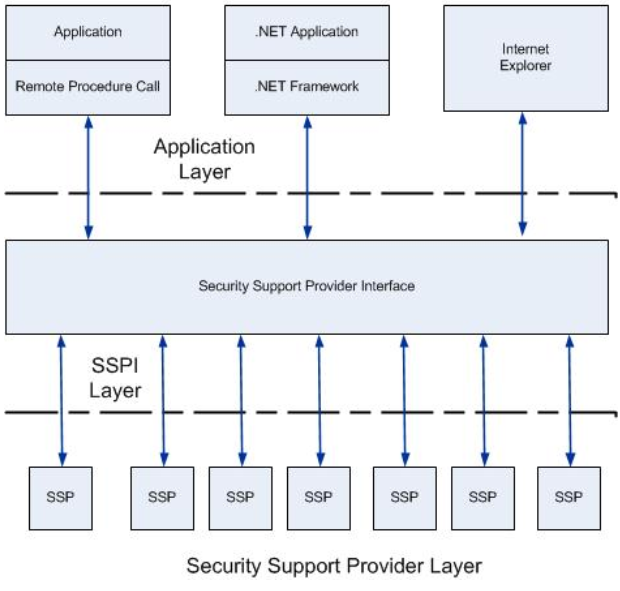
\includegraphics[width=\linewidth]{windows_knowledge/authentication/images/sspi.png}
  \caption{SSPI Architecture}
  \label{fig:sspi-architecture}
\end{figure}


The following sections describe the default SSPs that interact with the SSPI. The SSPs are used in different ways in Windows operating systems to promote secure communication in an unsecure network environment.

\subsection{Security Support Providers}
\subsubsection{Kerberos}
This SSP uses only the Kerberos version 5 protocol as implemented by Microsoft. This protocol is based on the Network Working Group's RFC 4120 and draft revisions. It is an industry standard protocol that is used with a password or a smart card for an interactive logon. It is also the preferred authentication method for services in Windows.

Because the Kerberos protocol has been the default authentication protocol since Windows 2000, all domain services support the Kerberos SSP. These services include:
\begin{itemize}
    \item Active Directory queries that use the Lightweight Directory Access Protocol (LDAP)
    \item Remote server or workstation management that uses the Remote Procedure Call service
    \item Print services
    \item Client-server authentication
    \item Remote file access that uses the Server Message Block (SMB) protocol (also known as Common Internet File System or CIFS)
    \item Distributed file system management and referral
    \item Intranet authentication to Internet Information Services (IIS)
    \item Security authority authentication for Internet Protocol security (IPsec)
    \item Certificate requests to Active Directory Certificate Services for domain users and computers
\end{itemize}

Location: \verb+%Windir%\System32\kerberos.dll+

\begin{itemize}
    \item \href{https://docs.microsoft.com/en-us/windows/win32/secauthn/microsoft-kerberos}{Microsoft Kerberos (Windows)}
    \item \href{https://docs.microsoft.com/en-us/windows/win32/secauthn/kerberos-ssp-ap}{Kerberos SSP/AP (Windows)}
    \item \href{https://docs.microsoft.com/en-us/previous-versions/windows/it-pro/windows-server-2003/cc739058(v=ws.10)}{Kerberos Authentication Technical Reference}
\end{itemize}

\subsubsection{NTLM}
The NTLM Security Support Provider (NTLM SSP) is a binary messaging protocol used by the Security Support Provider Interface (SSPI) to allow NTLM challenge-response authentication and to negotiate integrity and confidentiality options. NTLM is used wherever SSPI authentication is used, including for Server Message Block or CIFS authentication, HTTP Negotiate authentication (for example, Internet Web Authentication), and the Remote Procedure Call service. The NTLM SSP includes the NTLM and NTLM version 2 (NTLMv2) authentication protocols.

The supported Windows operating systems can use the NTLM SSP for the following:

\begin{itemize}
    \item Client/server authentication
    \item Print services
    \item File access by using CIFS (SMB)
    \item Secure Remote Procedure Call service or DCOM service
\end{itemize}
Location: \verb+%Windir%\System32\msv1_0.dll+

This provider is included by default in versions designated in the Applies to list at the beginning of this topic, plus Windows Server 2003 and Windows XP.

\begin{itemize}
    \item \url{https://docs.microsoft.com/en-us/windows/win32/secauthn/msv1-0-authentication-package}
    \item \url{https://docs.microsoft.com/en-us/windows/win32/secauthn/microsoft-ntlm}
    \item \url{https://docs.microsoft.com/en-us/previous-versions/windows/it-pro/windows-server-2008-R2-and-2008/jj865674(v=ws.10)}
\end{itemize}

\subsubsection{Digest}
Digest authentication is an industry standard that is used for Lightweight Directory Access Protocol (LDAP) and web authentication. Digest authentication transmits credentials across the network as an MD5 hash or message digest.

Digest SSP (Wdigest.dll) is used for the following:
\begin{itemize}
    \item Internet Explorer and Internet Information Services (IIS) access
    \item LDAP queries
\end{itemize}
Location: \verb+%Windir%\System32\Wdigest.dll+

This provider is included by default in versions designated in the Applies to list at the beginning of this topic, plus Windows Server 2003 and Windows XP.
\begin{itemize}
    \item \href{https://learn.microsoft.com/en-us/windows/win32/secauthn/the-digest-access-protocol}{The Digest Access Protocol}
    \item \href{https://docs.microsoft.com/en-us/windows/win32/secauthn/microsoft-digest-ssp}{[MS-DPSP]: Digest Protocol Extensions}
\end{itemize}

\subsubsection{Schannel}

Schannel, Window's security support provider for TLS/SSL connections, handles client authentication by allowing a remote server to verify the connecting user's identity. This process relies on PKI, using certificates as the main credential. During the TLS handshake, the server requests the client's certificate for authentication. The client, equipped with a CA-issued client authentication certificate trusted by the server, sends it over. Upon validation by the server, assuming all is well, access is granted.

Initially, Schannel tries to link the credential to a user account using Kerberos's \verb+S4U2Self+ feature. If that fails, it attempts to associate the certificate with a user account using various methods outlined in the \href{https://learn.microsoft.com/en-us/openspecs/windows_protocols/ms-rcmp/d16ed463-f75d-47f5-b19f-e026bcf1bffe}{Remote Certificate Mapping Protocol (MS-RCMP) specification}, such as the certificate's SAN extension or a combination of subject and issuer fields.

In default settings, only a few protocols in an Active Directory environment support authentication through Schannel immediately. While WinRM, RDP, and IIS can employ Schannel for client authentication, additional setup is necessary. However, LDAPS (LDAP over SSL/TLS) commonly works assuming Active Directory Certificate Services is configured.


The Secure Channel (Schannel) is used for web-based server authentication, such as when a user attempts to access a secure web server.

The TLS protocol, SSL protocol , the Private Communications Technology (PCT) protocol, and the Datagram Transport Layer (DTLS) protocol are based on public key cryptography. Schannel provides all these protocols. All Schannel protocols use a client/server model. The Schannel SSP uses public key certificates to authenticate parties. When authenticating parties, Schannel SSP selects a protocol in the following order of preference:
\begin{itemize}
    \item Transport Layer Security (TLS) version 1.0
    \item Transport Layer Security (TLS) version 1.1
    \item Transport Layer Security (TLS) version 1.2
    \item Secure Socket Layer (SSL) version 2.0
    \item Secure Socket Layer (SSL) version 3.0
    \item Private Communications Technology (PCT)
    \item Note PCT is disabled by default.
\end{itemize}

The protocol that is selected is the preferred authentication protocol that the client and the server can support. For example, if a server supports all the Schannel protocols and the client supports only SSL 3.0 and SSL 2.0, the authentication process uses SSL 3.0.

DTLS is used when explicitly called by the application. For more information about DTLS and the other protocols that are used by the Schannel provider, see Schannel Security Support Provider Technical Reference.

Location: \verb+%Windir%\System32\Schannel.dll+

This provider is included by default in versions designated in the Applies to list at the beginning of this topic, plus Windows Server 2003 and Windows XP.
\begin{itemize}
    \item \href{https://docs.microsoft.com/en-us/windows/win32/secauthn/secure-channel}{Secure Channel (Windows)}
    \item \href{https://docs.microsoft.com/en-us/previous-versions/windows/it-pro/windows-server-2003/cc784149(v=ws.10)}{TLS/SSL Technical Reference}
    \item \href{https://learn.microsoft.com/en-us/openspecs/windows_protocols/ms-tlsp/58aba05b-62b0-4cd1-b88b-dc8a24920346}{[MS-TLSP]: Transport Layer Security (TLS) Profile}
\end{itemize}


\subsubsection{Negotiate (SPNEGO)}
\label{windows:spnego}
The Simple and Protected GSS-API Negotiation Mechanism (SPNEGO) forms the basis for the Negotiate SSP, which can be used to negotiate a specific authentication protocol. When an application calls into SSPI to log on to a network, it can specify an SSP to process the request. If the application specifies the Negotiate SSP, it analyzes the request and picks the appropriate provider to handle the request, based on customer-configured security policies.

SPNEGO is specified in RFC 2478.

In supported versions of the Windows operating systems, the Negotiate security support provider selects between the Kerberos protocol and NTLM. Negotiate selects the Kerberos protocol by default unless that protocol cannot be used by one of the systems involved in the authentication, or the calling application did not provide sufficient information to use the Kerberos protocol.

Location: \verb+%Windir%\System32\lsasrv.dll+

This provider is included by default in versions designated in the Applies to list at the beginning of this topic, plus Windows Server 2003 and Windows XP.

\begin{itemize}
    \item \href{https://docs.microsoft.com/en-us/windows/win32/secauthn/microsoft-negotiate}{Microsoft Negotiate}
    \item \href{https://learn.microsoft.com/en-us/openspecs/windows_protocols/ms-spng/f377a379-c24f-4a0f-a3eb-0d835389e28a}{[MS-SPNG]: Simple and Protected GSS-API Negotiation Mechanism (SPNEGO) Extension}
    \item \href{https://learn.microsoft.com/en-us/openspecs/windows_protocols/ms-n2ht/4b88aa77-4b12-4933-8740-0f32d8f4eacf}{[MS-N2HT]: Negotiate and Nego2 HTTP Authentication Protocol}
\end{itemize}


\subsubsection{Credential (CredSSP)}
The Credential Security Service Provider (CredSSP) provides a single sign-on (SSO) user experience when starting new Terminal Services and Remote Desktop Services sessions. CredSSP enables applications to delegate users' credentials from the client computer (by using the client-side SSP) to the target server (through the server-side SSP), based on the client's policies. CredSSP policies are configured by using Group Policy, and the delegation of credentials is turned off by default.

Location: \verb+%Windir%\System32\credssp.dll+

This provider is included by default in versions designated in the Applies to list at the beginning of this topic.


CredSSP qui met également en oeuvre TLS pour transporter une
authentification basée sur SPNEGO et la délégation des in-
formations d'identification. CredSSP fait appel à
d'autres SSP : Negotiate pour la négociation SPNEGO, (qui lui-
même fait appel à NTLM ou Kerberos) et TSSSP 27 pour la déléga-
tion.

\begin{itemize}
    \item \href{https://docs.microsoft.com/en-us/openspecs/windows_protocols/ms-cssp/85f57821-40bb-46aa-bfcb-ba9590b8fc30}{[MS-CSSP]: Credential Security Support Provider (CredSSP) Protocol Specification}
    \item \href{https://learn.microsoft.com/en-us/previous-versions/windows/it-pro/windows-vista/cc749211(v=ws.10)}{Credential Security Service Provider and SSO for Terminal Services Logon}
\end{itemize}

\subsubsection{Negotiate Extensions (NegoExts)}
Negotiate Extensions (NegoExts) is an authentication package that negotiates the use of SSPs, other than NTLM or the Kerberos protocol, for applications and scenarios implemented by Microsoft and other software companies.

This extension to the Negotiate package permits the following scenarios:

\begin{itemize}
    \item Rich client availability within a federated system. Documents can be accessed on SharePoint sites, and they can be edited by using a full-featured Microsoft Office application.
    \item Rich client support for Microsoft Office services. Users can sign in to Microsoft Office services and use a full-featured Microsoft Office application.
    \item Hosted Microsoft Exchange Server and Outlook. There is no domain trust established because Exchange Server is hosted on the web. Outlook uses the Windows Live service to authenticate users.
    \item Rich client availability between client computers and servers. The operating system's networking and authentication components are used.
\end{itemize}

The Windows Negotiate package treats the NegoExts SSP in the same manner as it does for Kerberos and NTLM. NegoExts.dll is loaded into the Local System Authority (LSA) at startup. When an authentication request is received, based on the request's source, NegoExts negotiates between the supported SSPs. It gathers the credentials and policies, encrypts them, and sends that information to the appropriate SSP, where the security token is created.

The SSPs supported by NegoExts are not stand-alone SSPs such as Kerberos and NTLM. Therefore, within the NegoExts SSP, when the authentication method fails for any reason, an authentication failure message will be displayed or logged. No renegotiation or fallback authentication methods are possible.

Location: \verb+%Windir%\System32\negoexts.dll+

This provider is included by default in versions designated in the Applies to list at the beginning of this topic, excluding Windows Server 2008 and Windows Vista.

\subsubsection{PKU2U}
\label{windows:pku2u}
The PKU2U protocol was introduced and implemented as an SSP in Windows 7 and Windows Server 2008 R2 . This SSP enables peer-to-peer authentication, particularly through the media and file sharing feature called HomeGroup, which was introduced in Windows 7 . The feature permits sharing between computers that are not members of a domain.

Location: \verb+%Windir%\System32\pku2u.dll+

This provider is included by default in versions designated in the Applies to list at the beginning of this topic, excluding Windows Server 2008 and Windows Vista.

Additional resources for the PKU2U protocol and the PKU2U SSP

\begin{itemize}
    \item \url{https://docs.microsoft.com/en-us/previous-versions/windows/it-pro/windows-server-2008-R2-and-2008/dd560662(v=ws.10)}
\end{itemize}

\subsection{Security Support Provider selection}
The Windows SSPI can use any of the protocols that are supported through the installed Security Support Providers. However, because not all operating systems support the same SSP packages as any given computer running Windows Server, clients and servers must negotiate to use a protocol that they both support. Windows Server prefers client computers and applications to use the Kerberos protocol, a strong standards-based protocol, when possible, but the operating system continues to allow client computers and client applications that do not support the Kerberos protocol to authenticate.

Before authentication can take place the two communicating computers must agree on a protocol that they both can support. For any protocol to be usable through the SSPI, each computer must have the appropriate SSP. For example, for a client computer and server to use the Kerberos authentication protocol, they must both support Kerberos v5. Windows Server uses the function EnumerateSecurityPackages to identify which SSPs are supported on a computer and what the capabilities of those SSPs are.

The selection of an authentication protocol can be handled in one of the following two ways:

\subsubsection{Single authentication protocol}
When a single acceptable protocol is specified on the server, the client computer must support the protocol specified or the communication fails. When a single acceptable protocol is specified, the authentication exchange takes place as follows:
\begin{enumerate}
    \item The client computer requests access to a service.

    \item The server replies to the request and specifies the protocol that will be used.

    \item The client computer examines the contents of the reply and checks to determine whether it supports the specified protocol. If the client computer does support the specified protocol, the authentication continues. If the client computer does not support the protocol, the authentication fails, regardless of whether the client computer is authorized to access the resource.
\end{enumerate}

\subsubsection{Negotiate option}
The negotiate option can be used to allow the client and server to attempt to find an acceptable protocol. This is based on the Simple and Protected GSS-API Negotiation Mechanism (SPNEGO). When the authentication begins with the option to negotiate for an authentication protocol, the SPNEGO exchange takes place as follows:

\begin{enumerate}
    \item The client computer requests access to a service.

    \item The server replies with a list of authentication protocols that it can support and an authentication challenge or response, based on the protocol that is its first choice. For example, the server might list the Kerberos protocol and NTLM, and send a Kerberos authentication response.

    \item The client computer examines the contents of the reply and checks to determine whether it supports any of the specified protocols.
    \begin{itemize}
        \item If the client computer supports the preferred protocol, authentication proceeds.

        \item If the client computer does not support the preferred protocol, but it does support one of the other protocols listed by the server, the client computer lets the server know which authentication protocol it supports, and the authentication proceeds.

        \item If the client computer does not support any of the listed protocols, the authentication exchange fails.
    \end{itemize}
\end{enumerate}

\subsection{links}

\begin{itemize}
    \item \href{https://learn.microsoft.com/en-us/windows-server/security/windows-authentication/security-support-provider-interface-architecture}{Security Support Provider Interface Architecture}
\end{itemize}